\chapter{Étude}

% Introduction

\section{Introduction}

\indent La nature a donné à l’homme et aux animaux complexes des organes qui leur permettent d’interpréter les différentes informations de leur environnement. Ces organes peuvent capter des grandeurs physiques qui sont envoyées au cerveau pour pouvoir interpréter les changements dans le monde qui nous entoure ; ce sont les sens. L’un des phénomènes physiques capté par nos organes est “les ondes”, tantôt mécaniques avec l’ouïe, tantôt électromagnétiques avec la vue, qui constituent les deux principaux sens de l’homme. Or ces sens ne captent qu’une infime partie de tout le spectre existant des ondes.


Malheureusement ces sens peuvent être endommagés, ce qui devient une contrainte pour la personne affectée. Selon \acrfull{who}, nviron 1,3 milliard de personnes vivrait avec une forme de déficience visuelle \cite{WHO-blindness-and-visual-impairment}, où, approximativement, 49.1 million d'eux sont aveugles \cite{number-of-blind}. Heureusement, il existe différentes techniques, outils et des technologies disponibles pour permettre aux handicapés de réaliser leurs activités quotidiennes.


Un des outils les plus utilisés est la canne blanche qui permet à l’utilisateur de détecter des obstacles qui se trouvent à un mètre de lui environ et, également, de déceler l’état du sol sur lequel ils marchent. Cependant, il existe encore des déficiences pour détecter des obstacles plus hauts ainsi que pour toucher les obstacles et les reconnaître. La technologie des capteurs nous permet d’identifier des grandeurs physiques et de les transformer en informations grâce à la connaissance des phénomènes physiques qui y interviennent. La compréhension des ondes a permis de développer des capteurs qui peuvent détecter des objets à distance grâce à l’analyse des échos reçus.

% La nature a donné à l’homme et aux animaux des organes complexes qui leurs permettent d’interpréter les différentes informations de leur environnement. Ces organes peuvent capter des grandeurs physiques qui sont envoyées au cerveau pour pouvoir interpréter les
% événements dans le monde qui nous entoure ; ce sont les sens. L’un des phénomènes
% physiques capté par nos organes sont “les ondes”, mécaniques avec l’ouïe, et lumineux avec la vue, qui constituent les deux principaux sens de l’homme. Or ces sens ne captent qu’une infime partie de tout le spectre existant des ondes. \\
% Malheureusement, ces sens peuvent être endommagés, ce qui devient une contrainte pour la personne affectée. \\
% Selon \acrfull{who}, environ 1,3 milliard de personnes vivrait avec une forme de déficience visuelle \cite{WHO-blindness-and-visual-impairment}, où, approximativement, 49.1 million d'eux sont aveugles \cite{number-of-blind}. Si à l’échelle mondiale, la majorité des maladies engendrant la perte de la vision pourraient être évitées, il n’en demeurerait pas moins une augmentation du nombre des déficients visuels dans tous les pays, qu’ils soient industrialisés ou non. Du fait de l’accroissement de la durée de vie la proportion de non-voyants est plus importante parmi les personnes âgées. La cécité de l’enfant est un problème important, et plus particulièrement dans les pays en voie de développement du fait du manque de diagnostic précoce qui permettrait d’éviter de nombreux cas. Ainsi, seulement 13\% des personnes déficientes visuelles vivent dans des pays développés, dans lesquels le diagnostique est effectué plus précocement engendrant un traitement plus rapide. Ces statistiques montrent toute l’importance du diagnostic précoce ainsi que l’impact des Recherches actuelles sur son traitement. \\
% Depuis des décennies, les recherches sur le handicap visuel ont fait émerger de nombreux dispositifs pour rendre plus accessible l’information écrite, l’informatique, le déplacement contrôlé d’un endroit à un autre (la navigation) et tout ce qui a trait aux fonctions assurées en temps normal par le système visuel. \\
% Les pouvoirs publics se sont beaucoup intéressés ces dernières années aux différents aspects de la vie d’une personne handicapée visuelle, du diagnostic à l’accessibilité. \\
% De nombreux projets ont vu le jour pour faciliter la mobilité des personnes en situation de handicap ainsi que leur accès à l’information pour une meilleure insertion dans la société. Ainsi de nombreux projets de recherche ont émergé ces dernières années, la législation s’est aussi intéressée au problème de l’insertion des personnes handicapées dans les études et le monde du travail ainsi que l’accessibilité des lieux publics. Malgré de nombreux investissements ponctuels dans les agglomérations pour rendre l’environnement accessible, ces installations nécessitent un coût de maintenance très élevé et sont parfois laissées à l’abandon. Une des questions que nous pouvons nous poser est de savoir s’il est préférable de créer des installations supplémentaires dans les agglomérations pour les rendre accessibles ou bien s’il est préférable de créer des outils personnels permettant de mieux appréhender l’environnement sans avoir à le modifier. \\
% Les équipements rendant les installations urbaines plus accessibles sont très utiles mais pour ces raisons, nous sommes convaincus de l’utilité de concevoir et de développer des systèmes de suppléance permettant de réduire les handicaps liés à la déficience visuelle, sans modifier l’environnement. \\
% Certaines aides comme la canne blanche ou le chien d’aveugle sont devenues des standards qui ont constitué de grandes avancées pour l’autonomie des personnes aveugles. Cependant, il existe encore des déficiences pour détecter des obstacles plus hauts ainsi que pour toucher les obstacles et les reconnaître. Une multitude d’aides électroniques ont été développées depuis les années 60, évoluant au gré des progrès de la miniaturisation des composants et des avancées technologiques .La technologie des capteurs nous permettent d’identifier des grandeurs physiques et de les transformer en informations grâce à la connaissance des phénomènes physiques qui y interviennent. La compréhension des ondes a permis de développer des capteurs qui peuvent détecter des objets à distance grâce à l’analyse des échos
% reçus. \\
% Ce mémoire a pour objectif d’augmenter l’autonomie des personnes non voyantes en restaurant leur faculté à localiser des objets visuels. \\
% Comment utiliser les propriétés des ondes pour rendre la détection des obstacles plus facile aux aveugles ? Dans un premier temps, nous donnerons des informations sur le fonctionnement et la réalisation du projet, puis dans un deuxième temps, nous parlerons des caractéristiques des ondes et des capteurs utilisés pour finalement étudier les éléments constitutifs de la canne et les différentes étapes de réalisation de cette dernière. 

% Problématique et besoins

\section{Problématique et besoins}

\todo[inline]{Problématique et besoins}

\section{Solutions et objectifs}

Comme indiqué précédemment, les aveugles ont du mal à faire leurs tâches quotidiennes simples, sans parler de pouvoir d'aller dehors. Ce qui nous a fait réfléchir à la façon dont nous pouvons faciliter leur navigation. Alors que les objectifs de notre projet sont les suivants:
\begin{itemize}
    \item La détection des obstacles et leur proximité.
    \item Faciliter l’utilisation du téléphone pour la navigation et la rendre plus rapide et plus facile.
    \item Être en mesure de trouver leur canne égarée à l’aide de leur téléphone, et vice versa.
    \item Appeler à l’aide au cas où il serait perdu, et généralement faciliter l’information des autres de leur emplacement actuel.
    \item Trouver les différents lieux proches de lui, classés par catégories, et l’y conduire.
    \item Contrôler toutes ces tâches avec son téléphone et/ou sa canne.
\end{itemize}

\section{Principe de fonctionnement}

\todo[inline]{Expliquer ce schéma avant}

\begin{figure}[!ht]
    \centering
    \includegraphics[width=15cm]{fig/schéma fonctionnelle.png}
    \caption{Schéma de fonctionnement globale du système}
\end{figure}

\FloatBarrier


\section{Les composants et technologies utilisé}

\subsection{Arduino}

\subsubsection{C'est Quoi un Arduino ?}
Arduino est une plateforme électronique open-source basée sur du matériel et des logiciels faciles à utiliser. Cartes Arduino sont capables de lire les entrées - lumière sur un capteur, un doigt sur un bouton, ou un message Twitter - et de le transformer en une sortie - activer un moteur, allumer une LED, publier quelque chose en ligne. Vous pouvez dire à votre carte quoi faire en envoyant un ensemble d’instructions au micro-contrôleur de la carte \cite{arduino-introduction}.

\subsubsection{Les différents types d'un Arduino ?}
Les Arduinos sont caractérisés par plusieurs caractéristiques:

\begin{itemize}
    \item Processeur
    \item Vitesse d'horloge
    \item Tension d'entrée
    \item Tension de sortie
    \item Mémoire de stockage (Flash Memory)
    \item Mémoire vive (\acrshort{RAM})
    \item Nombre des pins entrée/sortie logique
    \item Nombre des pins entrée/sortie analogique
    \item Nombre des convertisseurs numérique/analogique (\acrshort{DAC})
    \item Nombre des pins supportant la modulation de largeur d'impulsion (\acrshort{PWM})
    \item Les différents protocoles de communication supportés (UART / SPI / I\(^2\)C)
    \item Type du connecteur
    \item Ses dimensions
\end{itemize}

Pour notre projet, on n'est pas très intéressé à toutes ses différentes caractéristiques, d'où on a créé un tableau qui compare les diffèrent types en se basant sur les caractéristiques qu'on a besoin.


\newcolumntype{C}[1]{ >{\centering\arraybackslash} m{#1} }
\begin{table}[hbt!]
    \centering
    \begin{tabular}{|C{3cm}|C{2cm}|C{2.2cm}|C{2.2cm}|C{1.2cm}|C{1.5cm}|C{1.2cm}|}%|c|c|c|c|c|c|c|
        \hline
        &&&&&&\\ % Adding empty space on top of 0th column
        & Modèle & Vitesse d'horloge & Mémoire de programme & RAM & Nombre des pins & PWM \\[18pt]
        \hline
        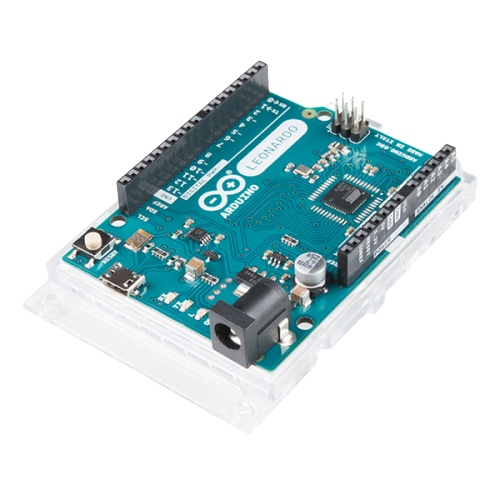
\includegraphics[width=3cm]{assets/arduino/leonardo.png} & UNO & 16MHz & 32KB & 2KB & 20 & 6 \\
        \hline
        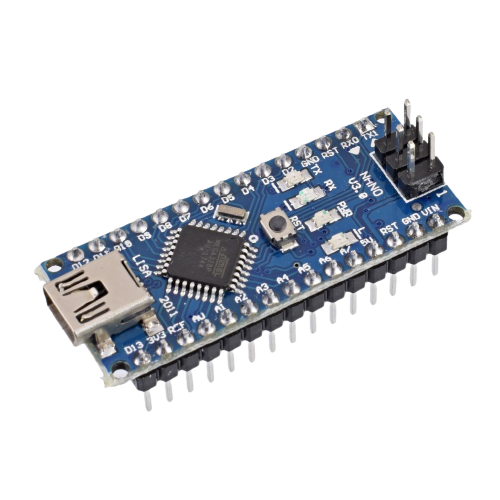
\includegraphics[width=3cm]{assets/arduino/nano.png} & Nano & 16MHz & 32KB & 2KB & 20 & 6 \\
        \hline
        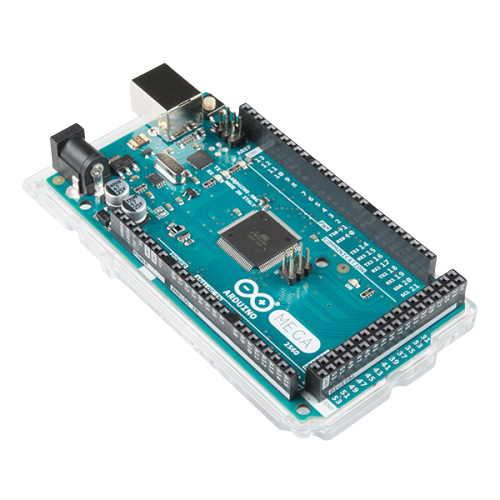
\includegraphics[width=3cm]{assets/arduino/mega.png} & Mega & 16MHz & 256KB & 8KB & 54 & 15 \\
        \hline
        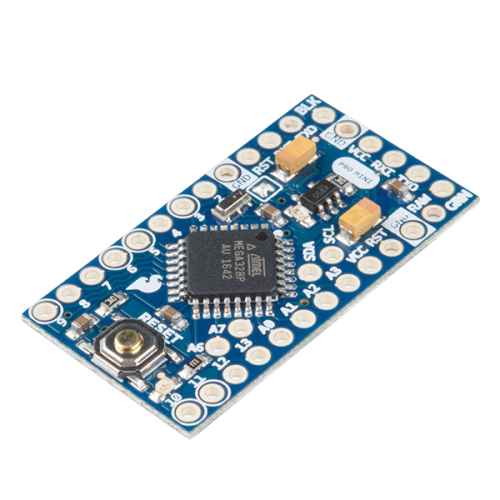
\includegraphics[width=3cm]{assets/arduino/pro mini.png} & Pro Mini & 8MHz & 32KB & 2KB & 22 & 8 \\
        \hline
        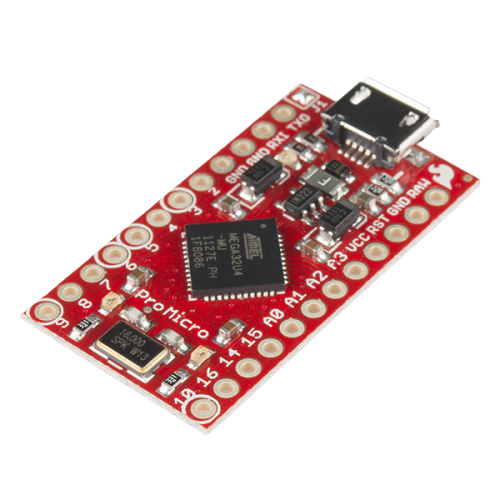
\includegraphics[width=3cm]{assets/arduino/pro micro.png} & Pro Micro & 16MHz & 32KB & 2.5KB & 18 & 5 \\
        \hline
        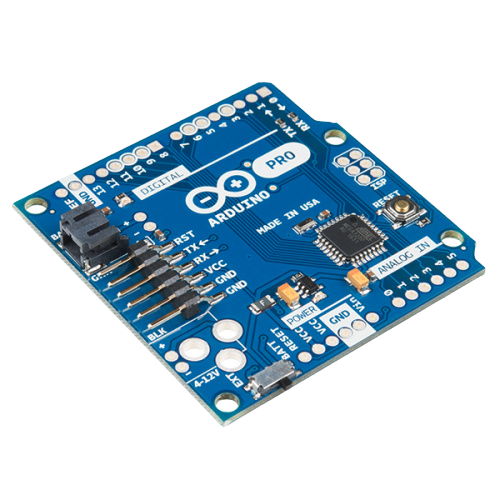
\includegraphics[width=3cm]{assets/arduino/pro.png} & Leonardo & 16MHz & 32KB & 2.5KB & 20 & 12 \\
        \hline
    \end{tabular}
    \caption{Les différents types d'Arduino \cite{arduino-types}}
\end{table}

\FloatBarrier

\subsubsection{Que-ce-qu'on a choisi?}

Notre projet a besoin de 14 entrées/sorties logiques, et une analogique. Où on avait le choix entre plusieurs modèles comme l'Arduino UNO, Nano, Pro Mini, et toute autre diffèrent type. Donc on avait pris autres caractéristiques en considération, surtout le prix et les dimensions, c'était indispensable d'avoir une qui peut être contenue dans un petit boîtier avec un bon prix. D'où on a choisi l'\textbf{Arduino Nano}, qu'il y avait des dimensions de 45 x 18 x 18 mm et un poids de 7g, à seulement 60DH.


\begin{figure}[hbt!]
    \centering
    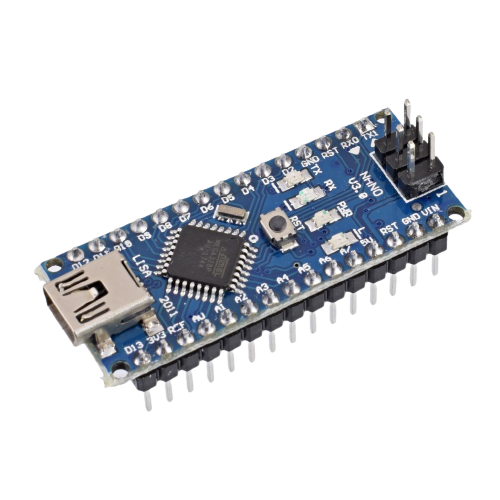
\includegraphics[width=5cm]{assets/arduino/nano.png}
    \caption{Arduino Nano}
\end{figure}

\subsection{Capteur de proximité HC-SR04}

\subsubsection{Description}

Le capteur de distance ultrasonique HC-SR04 est un capteur utilisé pour détecter la distance d’un objet à l’aide d’un sonar. Il est idéal pour tous les projets de robotique que vous avez qui vous obligent à éviter les objets, en détectant à quel point ils sont proches, vous pouvez vous éloigner d’eux \cite{piborg-hc-sr04}!

\subsubsection{Avantages}
Le capteur est petit, facile à utiliser dans n’importe quel projet de robotique et offre une excellente détection sans contact entre 2 cm à 400 cm avec une précision de 3mm. Puisqu’il fonctionne sur 5 volts, il peut être raccordé directement à un Arduino ou tout autre microcontrôleur logique 5V.

\subsubsection{Principe de fonctionnement}
Tout commence lorsqu’une impulsion d’au moins 10 µs (10 microsecondes) de durée est appliquée à la broche de déclenchement (Trigger). En réponse à cela, le capteur transmet une rafale sonore de huit impulsions à 40 KHz. Ce motif à 8 impulsions rend la « signature ultrasonique » de l’appareil unique, ce qui permet au récepteur de différencier le motif transmis du bruit ultrasonique ambiant.

Les huit impulsions ultrasoniques se déplacent dans l’air loin du transmetteur. Pendant ce temps, la broche Echo va HAUT pour commencer à former le début du signal d’écho-retour.

Dans le cas, si ces impulsions ne sont pas réfléchies en arrière, le signal Echo expire après 38 ms (38 millisecondes) et revient bas. Ainsi, une impulsion de 38 ms n’indique aucune obstruction dans la plage du capteur \cite{hcsr04}.

On peut calculer la distance entre le capteur et l'objet en utilisant la simple relation en fonction de la vitesse du sons et la durée de déclenchement: \[d=\frac{v}{2 \cdot t} \ \text{où} \ v \approx 340 m/s\]


\begin{figure}[hbt!]
    \centering
    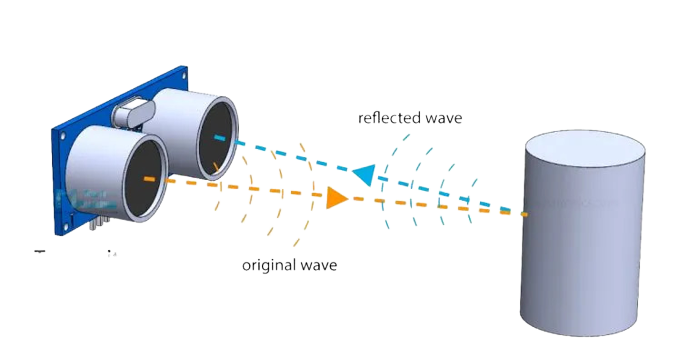
\includegraphics[width=14cm]{assets/HC-SR04/principe 3d.png}
\end{figure}

\begin{figure}[hbt!]
    \centering
    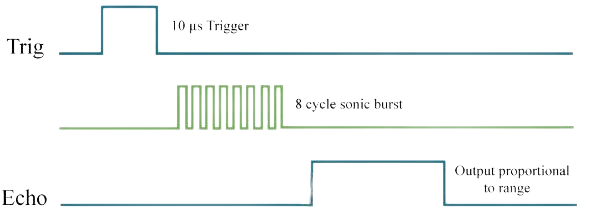
\includegraphics[width=14cm]{assets/HC-SR04/principe.png}
    \caption{Principe du fonctionnement du HC-SR04}
\end{figure}

\begin{figure}[!htbp]
    \centering
    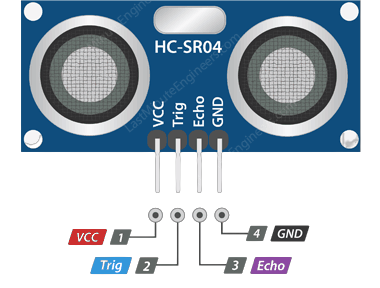
\includegraphics[width=10cm]{assets/HC-SR04/pinout.png}
    \caption{Brochage du module SR-HC04}
\end{figure}

\FloatBarrier

\subsection{Module Bluetooth: HC-05}

\subsubsection{Description}
Le module HC-05 est un module Bluetooth SPP (Serial Port Protocol), ce qui signifie qu’il communique avec l’Arduino via la communication série

\begin{figure}[!htbp]
    \centering
    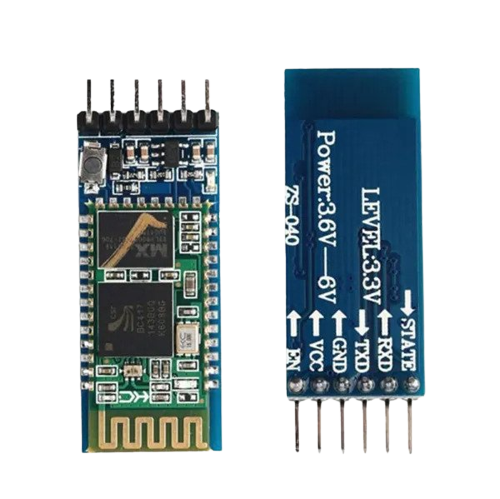
\includegraphics[width=8cm]{assets/HC-05/pinout.png}
    \caption{Module Bluetooth HC-05}
\end{figure}

\FloatBarrier

\subsubsection{Brochage}
Le HC-05 consiste 6 broches:
\begin{itemize}
    \item VCC et GND: Pour l'alimentation +5V
    \item TXD et RXD: Pour la communication série
    \item State: Signifie si le module et connecter en Bluetooth ou pas. HIGH si oui, LOW si non.
    \item Enable: Broche de configuration, on la met a l'état HIGH pour avoir la possibilité de configurer le module (Nom, Mot de passe, Type ...) avec la communication série.
\end{itemize}

\subsection{Les vibreur et le Motor Driver L293D}

\subsubsection{Vibreur}

Pour avertir l'utilisateur de la proximité d'objets devant lui, on va utiliser deux vibreurs situés à chaque côté de notre cane.

\begin{figure}[!htbp]
    \centering
    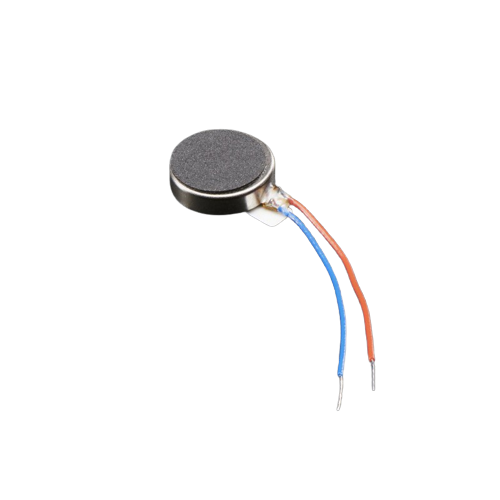
\includegraphics[width=8cm]{assets/vibrator.png}
    \caption{Moteur Vibreur}
\end{figure}

\FloatBarrier

Ce type de vibreurs nécessite 80mA et 5V pour bien fonctionner, main l'Arduino nano a une limitation de 40mA par broche, d'où on a besoin d'un motor driver.

\subsubsection{Motor Driver L293D}
Le circuit intégré L293D permet de piloter 2 moteurs à courant courant continu dans les deux sens de rotation et pour faire de la variation de vitesse.

\begin{figure}[!htbp]
    \centering
    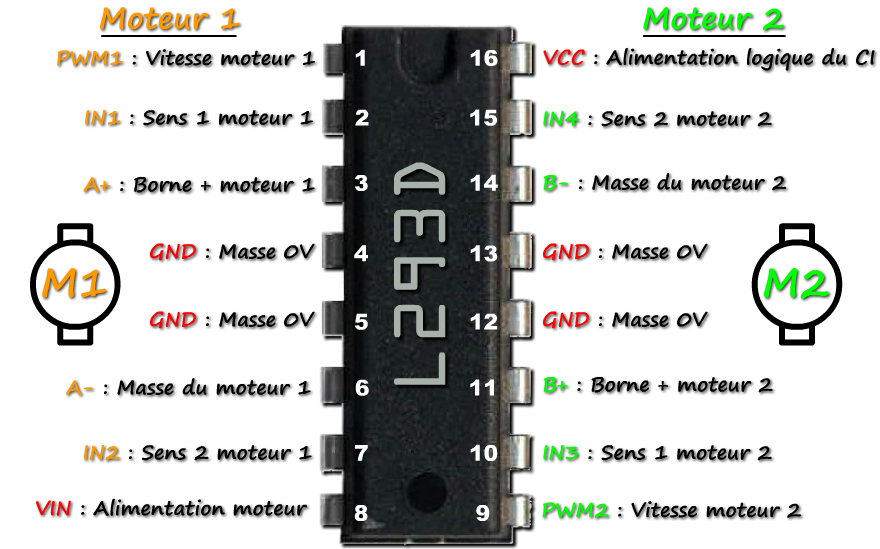
\includegraphics[width=14cm]{assets/L293D/pinout.png}
    \caption{Brochage du driver moteur L293D \cite{l293d-electrotoile}}
\end{figure}

\FloatBarrier

Pour notre projet, on n'a pas besoin de tourner le moteur à deux sens, donc on peut utiliser jusqu'à 4 moteurs.

\subsection{Bipeur (Buzzer)}
Un buzzer (anglicisme) ou bipeur est un élément électromécanique ou piézoélectrique qui produit un son caractéristique quand on lui applique une tension : le bip. Certains nécessitent une tension continue, d'autres nécessitent une tension alternative \cite{frwiki:178425382e}.

\begin{figure}[!htbp]
    \centering
    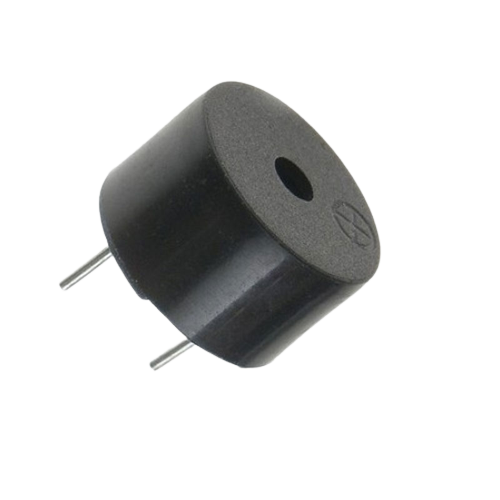
\includegraphics[width=8cm]{assets/buzzer.png}
    \caption{Buzzer}
\end{figure}

\FloatBarrier

\subsection{Flutter}

Flutter est un kit de développement logiciel (SDK) d'interface utilisateur open-source créé par Google. Il est utilisé pour développer des applications pour Android, iOS, Linux, Mac, Windows, Google Fuchsia et le web à partir d'une seule base de code \cite{frwiki:192185851}.

\begin{figure}[!htbp]
    \centering
    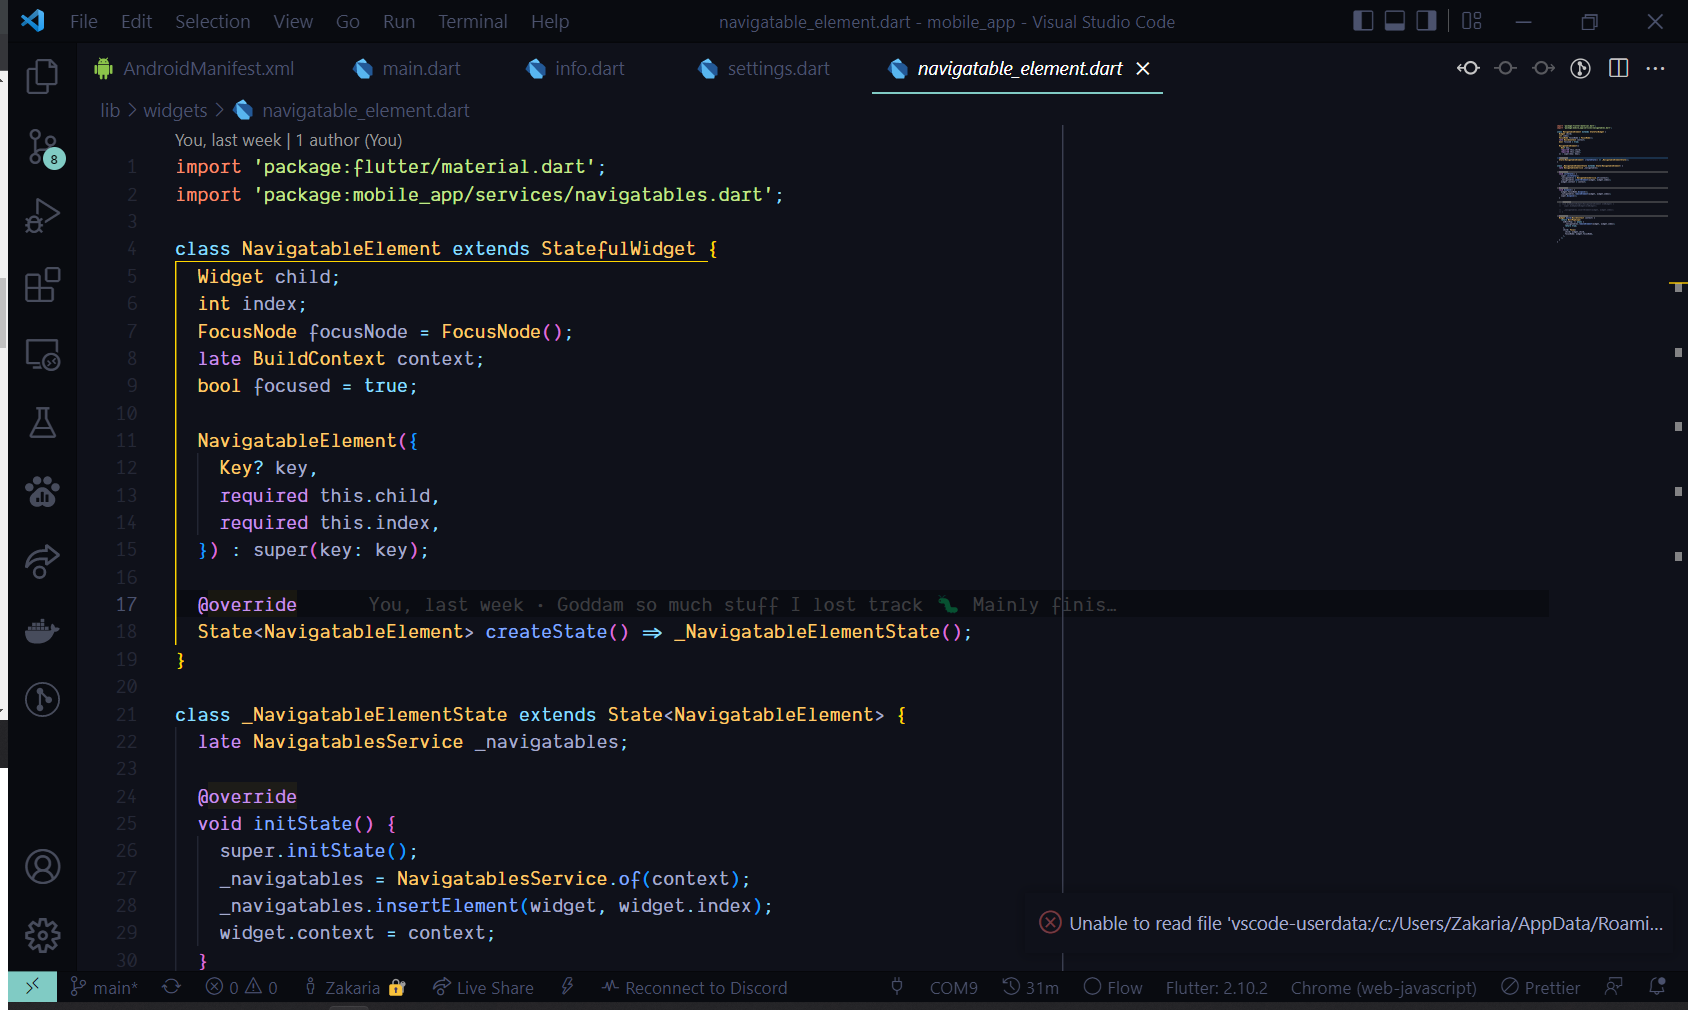
\includegraphics[width=\linewidth]{assets/flutter/example code.jpg}
    \caption{Code exemple du Flutter extrait de notre application}
\end{figure}

\begin{figure}[!htbp]
    \centering
    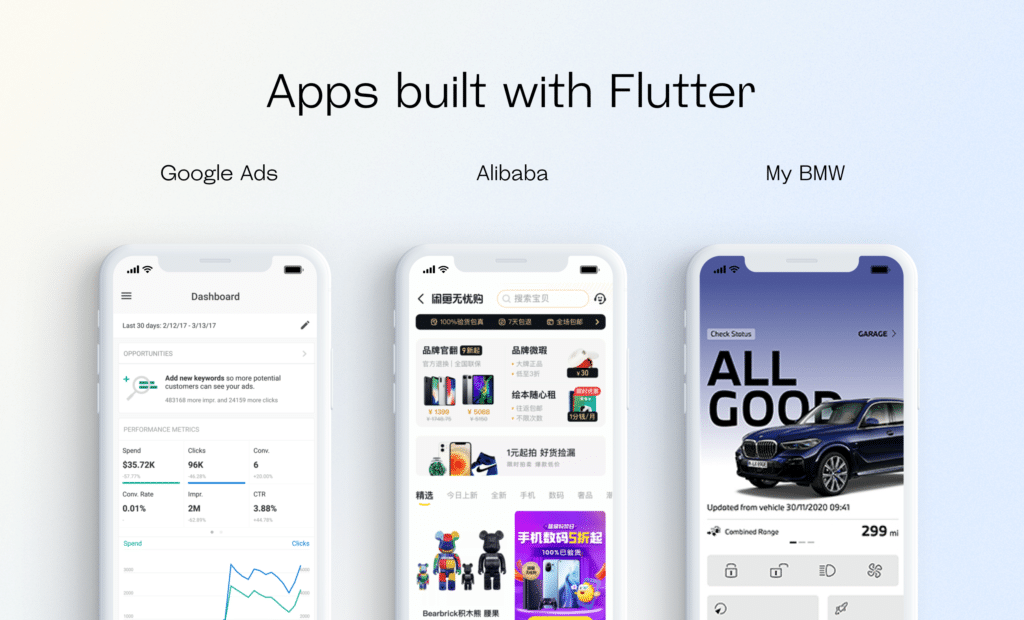
\includegraphics[width=.8\linewidth]{assets/flutter/example-apps-built-with-flutter.png}
    \caption{Des application qui sont aussi faites avec Flutter}
\end{figure}

\FloatBarrier

\subsection{L'accessibilité et les lecteurs d'écran}

\subsubsection{L'accessibilité}

\paragraph{Définition}

L’accessibilité est le concept selon lequel un produit ou un service peut être utilisé par tout le monde, peu importe la façon dont il est utilisé. Il existe des lois sur l’accessibilité pour aider les personnes handicapées, mais les concepteurs devraient de toute façon essayer d’accommoder tous les utilisateurs potentiels dans de nombreux contextes d’utilisation. Pour ce faire, il y a des avantages solides, notamment une meilleure conception pour tous \cite{what-is-accessibility}.

\paragraph{Pourquoi je dois l'implémenter ?}

L’accessibilité est non seulement la bonne chose à faire, mais apporte souvent aussi des avantages à tous les utilisateurs. C’est parce que les caractéristiques d’accessibilité qui aident les personnes handicapées aident souvent d’autres personnes aussi. Par exemple, les sous-titres vidéo qui aident les personnes ayant des difficultés auditives aident également une personne qui regarde la vidéo en mode muet (p. ex., dans un fil de médias sociaux). Un texte lisible et contrasté qui aide les personnes ayant des problèmes de vision aide également les personnes ayant une vision parfaite qui utilisent l’application à l’extérieur en plein soleil. De nombreux utilisateurs, quelles que soient leurs capacités, seront confrontés à des défis en raison de contextes exigeants \cite{what-is-accessibility}.
%Lorsque vous concevez pour tous les niveaux de capacité, vous pouvez créer des produits et des services que tout le monde peut utiliser et apprécier, ou du moins trouver utile ou apaisant .

Dans notre cas, puisque notre application sera principalement utilisée avec des personnes ayant une déficience visuelle, il est essentiel que notre application soit accessible.


\subsubsection{Les lecteurs d'écran (Screen Readers)}